\chapter{Models and Methods} \label{sec:ch_methods}

\section{Manual Design of Extraction Rules} \label{sec:methods_manual}
\graphicspath{{../img/ch50/}}

In this section, the extraction method based on manually created linguistic rules will be described. First of all a data flow schema of the extraction process will be presented. Then a description of several stages of evolution of the method will demonstrate how this method came to its existence and which decisions stood behind the development and the final implementation, which will be described in the next chapter.

The approach is based on linguistic preprocessing, oriented to text structured to individual sentences. 



%%%%%%%%%%%%%%%%%%%%%%%%%%%%%%%%%%%%%%%%%%%%%%%%%%%%%%%%%%%%%%%%%%%%%%%%%%%%%%%%%%%%%
\subsection{Data Flow} \label{sec:ch50_data_flow}
%%%%%%%%%%%%%%%%%%%%%%%%%%%%%%%%%%%%%%%%%%%%%%%%%%%%%%%%%%%%%%%%%%%%%%%%%%%%%%%%%%%%%

\begin{figure}
	\centering
		\includegraphics[width=0.2\hsize]{ap_schema}
	\caption{Schema of the extraction process.}
	\label{fig:ch50_ap_schema}
\end{figure}


\begin{figure}
	\centering
		\includegraphics[width=0.5\hsize]{article}
	\caption{One web page with an accident report.}
	\label{fig:ch50_article}
\end{figure}


The method was designed as a method for extraction of information from web resources. Thus the extraction process starts on the Web. On the other hand the method was intended to serve the evolution of the Semantic Web, so the final goal of the extraction process is the extracted information stored in the form of a semantic web ontology. A schema in Figure~\ref{fig:ch50_ap_schema} splits the process into four steps (phases) among five media types. The schema does not cover the extraction rules design phase; it is assumed that extraction rules were already designed by a human designer; Section~\ref{sec:ch50_rules_design} provides details about that. A description of individual steps follows. 



\begin{enumerate}
\item \emph{Extraction of text} \\ First of all, target web pages have to be identified, downloaded and text has to be extracted form them. This issue is not studied in the present work. A RSS feed of the fire department web-site was used to identify and download relevant pages and the desired text (see highlighted area in the Figure~\ref{fig:ch50_article}) was extracted by means of a regular expression. The text is an input of the second phase.

\item \emph{Linguistic annotation} \\ In this phase the extracted text is processed by several linguistic tools. The tools analyze the text and produce corresponding set of linguistic dependency trees. There is a rich choice of linguistic tools available (see Section~\ref{sec:ch30_ling_tools}), but only PDT based tools were used in illustration examples and linguistic trees are always of the form of Tectogrammatical trees, but note that the method is general and it is not limited to the PDT presentation of linguistic dependency trees.

\item \emph{Data extraction} \\ The structure of linguistic dependency trees is used for the extraction of relevant structured data form the text. The extraction method used in this phase is the main topic of this section (Section~\ref{sec:methods_manual}) and details about the method are discuses in following subsections.

\item \emph{Semantic representation} \\ Although the output of the previous phase is already of a structured form, it is not necessarily of the form of a semantic web ontology. The output has to be converted to some ontology format (RDF, OWL) and appropriate schema for given domain and type of extracted information. 

This last step of the extraction process represents a logical distinction between two functionally different tasks of the extraction method. The first task represented by the previous (Data extraction) phase is responsible for choosing of ``what’’ should be extracted, while the second task (Semantic representation) should determine what to do with the extracted data or how to formulate the pieces of information discovered by the Data extraction phase. The border between these two tasks is rather vague and they could be merged together, but we think that the distinction between them can help to understand the problem better.


In the present work only a design of this phase is provided (with a small exception -- using shareable extraction ontologies, see Section~\ref{sec:methods_Shareable_Extraction_Ontologies}) because: (1) this task seems to be strongly dependent on manual work of human designers and (2) its potential for meaningful scientific investigation seems to be rather small. Details about this step are further discussed in Section~\ref{sec:ch50_sem_interpret}.
\end{enumerate}



%%%%%%%%%%%%%%%%%%%%%%%%%%%%%%%%%%%%%%%%%%%%%%%%%%%%%%%%%%%%%%%%%%%%%%%%%%%%%%%%%%%%%
\subsection{Evolution of the Method}
%%%%%%%%%%%%%%%%%%%%%%%%%%%%%%%%%%%%%%%%%%%%%%%%%%%%%%%%%%%%%%%%%%%%%%%%%%%%%%%%%%%%%

Our first attempt to extract some structured data from linguistically annotated text was done in a standard procedural programming environment (more precisely in Perl, Btred). After an initial phase of development first extraction rule was created as a single executable procedure. This procedure will be described in the next chapter (Section~\ref{sec:impl_btred_rules}) and listed in Figure~\ref{lst:btred_rule}. There are many drawbacks of the procedural rule design: such extraction rules are difficult to read, tedious to create, error prone, graphical or assisted design is impossible. On the other hand, this approach has the advantage of the programming language proximity. When a designer designs a procedural extraction rule he or she actually codes it in a procedural programming language and it is easy to add some additional functionality that will be executed and evaluated along with the extraction rule. Thus the designer has the full power of the programming language in hand and he or she can use it inside of the extraction rule. This possibility will be discussed later in the context of semantic interpretation of extracted data.

Dissatisfaction from tedious and time consuming design of procedural extraction rules led us to the idea of a special rule language. We were looking for a language that would allow expressing tree patterns and consequent extraction actions of extraction rules. It turned out that the Netgraph query language is very suitable for the first purpose -- expressing tree patterns. An extension of the Netgraph query language to a language for extraction rules was quite simple then. See the details in the next section.

Last two steps in the evolution of the extraction method were (1) creation of machine learning procedure that is capable to learn extraction rules from manually annotated corpus (see in Section~\ref{sec:methods_learning}) and (2) possibility to export extraction rules to a shareable extraction ontology so the extraction rules can be evaluated on a document by an ordinary semantic web reasoner outside of the original extraction tool (see in Section~\ref{sec:methods_Shareable_Extraction_Ontologies}).


%%%%%%%%%%%%%%%%%%%%%%%%%%%%%%%%%%%%%%%%%%%%%%%%%%%%%%%%%%%%%%%%%%%%%%%%%%%%%%%%%%%%%
\subsection{Netgraph Based Extraction Rules}
%%%%%%%%%%%%%%%%%%%%%%%%%%%%%%%%%%%%%%%%%%%%%%%%%%%%%%%%%%%%%%%%%%%%%%%%%%%%%%%%%%%%%

\begin{figure}
	\centering
		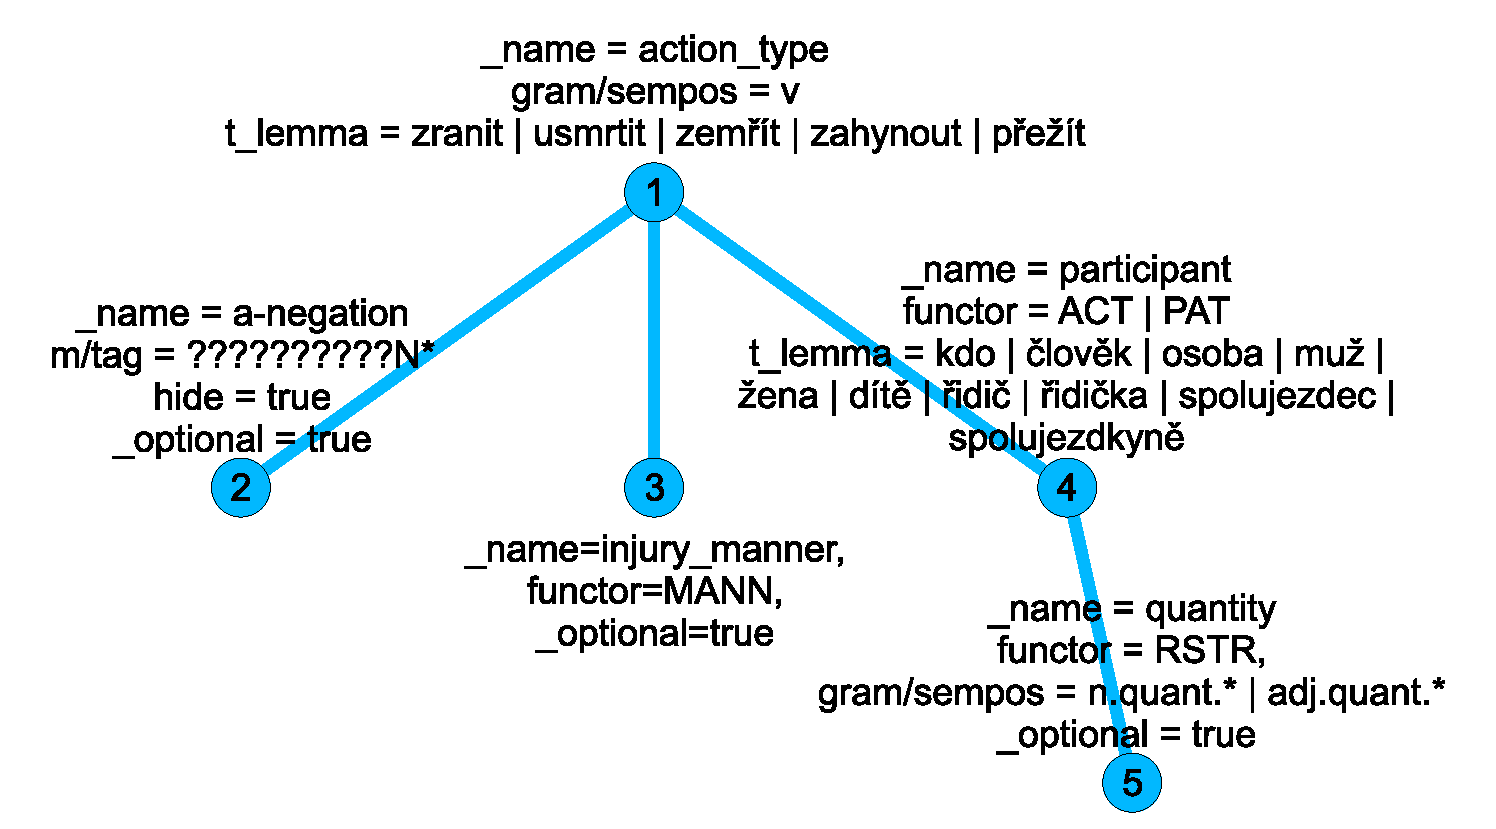
\includegraphics[width=0.5\hsize]{extract_patern}		
\\Transcript:\\
\begin{tabular}{|c|c|c|c|c|}
\hline
zranit & usmrtit & zemřít & zahynout & přežít\\
to injure & to kill & to die & to wane & to survive\\
\hline
\end{tabular}
\\\begin{tabular}{|c|c|c|c|c|c|}
\hline
kdo & člověk & osoba & muž & žena & dítě\\
somebody & (hu)man & person & man & woman & child\\
\hline
\end{tabular}
\\\begin{tabular}{|c|c|c|c|}
\hline
řidič & řidička & spolujezdec & spolujezdkyně\\
driver & woman driver & passenger & woman passenger\\	
\hline
\end{tabular}		
	\caption{A manually created extraction rule investigating numbers of injuries and fatalities.}
	\label{fig:ch50_extract_patern}
\end{figure}



Netgraph based extraction rules are declarative, they do not specify a sequential procedure ``what to do with a linguistic tree'', they are rather based on conditions and selections similar to SQL.

Netgraph is a linguistic tool used for searching through a syntactically annotated corpus (see Section~\ref{sec:ch30_netgraph} for details). Netgraph queries are written in a special query language with a graphical representation. The graphical representation of a query is much better readable than its linear textual representation and we will use the graphical representation only. Figure~\ref{fig:ch50_extract_patern} shows an example Netgraph query. It specifies necessary tree structure that has to be present in a matching tree and attribute restrictions that have to hold true for corresponding nodes (the restrictions are printed beside the nodes).



We adopted Netgraph queries and extended them to extraction rules that can be written in following pseudo SQL SELECT form:

\begin{minted}{sql}
SELECT node1_name.attr1_name, node2_name.attr2_name, ... FROM netgraph_query
\end{minted}

where \emph{netgraph\_query} stands for an arbitrary Netgraph query, \emph{node1\_name}, \emph{node2\_name}, etc. stand for individual names of nodes defined in \emph{netgraph\_query} and \emph{attr1\_name}, \emph{attr2\_name}, etc. stand for names of linguistic attributes whose values should be picked out from the corresponding matching tree nodes.

The extraction works as follows: the Netgraph query is evaluated by searching through a corpus of linguistic trees. Matching trees are returned and the desired information defined by the SELECT part of the extraction rule is taken from particular tree nodes and printed to the output.

Let us explain the extraction procedure in detail, using the example of extraction rule from the Figure~\ref{fig:ch50_extract_patern}, which is looking for information about killed and injured people during a (usually car) accident. This rule consists of five nodes. Each node of the rule will match with the corresponding node in each matching tree. So we can investigate the relevant information by reading values of linguistic attributes of matching nodes. We can find out the number (node number 5) and kind (4) of people, which were or were not (2) killed or injured (1) by an accident that is presented in the given sentence. And we can also identify the manner of injury (light or heavy) in the node number 3.

Implementation details and some additional examples of these extraction rules will be presented in the next chapter (Section~\ref{sec:impl_manual_rules}).



%%%%%%%%%%%%%%%%%%%%%%%%%%%%%%%%%%%%%%%%%%%%%%%%%%%%%%%%%%%%%%%%%%%%%%%%%%%%%%%%%%%%%
\subsection{Methodology for Rule Designers} \label{sec:ch50_rules_design}
%%%%%%%%%%%%%%%%%%%%%%%%%%%%%%%%%%%%%%%%%%%%%%%%%%%%%%%%%%%%%%%%%%%%%%%%%%%%%%%%%%%%%

\begin{figure}
	\centering
		\includegraphics[angle=-90, width=0.5\hsize]{coverge_tuning}
	\caption{Gradual refinement of an extraction rule.}
	\label{fig:ch50_coverge_tuning}
\end{figure}


The process of manual design of extraction rules is heavily dependent on skills and experience of a human designer and fulfillment of the process is quite creative task. In this section we try to pick it up as precisely as possible because we assume that a formal description of this process can help in two ways. First -- a new designer can use it as a cook book and progress more quickly. Second -- it can help with development of tools for assisted rule design. We will concentrate on the Netgraph based extraction rules because we think they are more useful.

The process consists of two parts: construction of a Netgraph query and semantic interpretation of the query. The semantic interpretation part will be discussed in the next section.

One obvious preposition of the procedure is that we have a collection of training texts.
The procedure is demonstrated in Figure~\ref{fig:ch50_coverge_tuning} and it starts with frequency analysis of words (their lemmas) occurring in the texts. Especially frequency analysis of verbs is very useful --- meaning of a clause is usually strongly dependent on the meaning of the corresponding verb.

\textbf{Frequency analysis} helps the designer to choose some representative words (\textbf{key-words}) that will be further used for searching the training text collection. Ideal choice of key-words would cover the majority of sentences that express the information we are looking for and it should cover minimal number of the not-intended sentences. An initial choice need not be always sufficient and the process could iterate.

Next step of the procedure consists in \textbf{investigating trees} that are covered by key-words. The designer is examining \textbf{matching trees} --- looking for positions of key-words and their \textbf{neighboring} nodes.

After that the designer can formulate an initial \textbf{Netgraph query} and he or she can compare result of the Netgraph query with the coverage of key-words. Based on this he or she can reformulate the query and gradually refine the query and \textbf{tune the query coverage}.

There are two goals of the query tuning. The first goal is maximization of the relevance of the query. An ideal result is a query that covers all sentences expressing given type of information and no other. The second goal is to involve all important tree-nodes to the query. The second goal is important because the \textbf{complexity of the query} (number of involved nodes) makes it possible to extract more complex information. For example see the query on the Figure~\ref{fig:ch50_extract_patern} --- each node keeps different kind of information.


%%%%%%%%%%%%%%%%%%%%%%%%%%%%%%%%%%%%%%%%%%%%%%%%%%%%%%%%%%%%%%%%%%%%%%%%%%%%%%%%%%%%%
\subsection{Semantic Interpretation of Extracted Data} \label{sec:ch50_sem_interpret}
%%%%%%%%%%%%%%%%%%%%%%%%%%%%%%%%%%%%%%%%%%%%%%%%%%%%%%%%%%%%%%%%%%%%%%%%%%%%%%%%%%%%%

After the designer has successfully formulated the Netgraph query he or she has to supply semantic interpretation of the query. This interpretation expresses how to transform matching nodes of the query (and the available linguistic information connected with the nodes) to the output data.

We did not talk about the extraction output so far. It will be described in the next chapter. For the current description, it is sufficient to say that both methods (the procedural one and the declarative one) have, although structured but still, proprietary XML extraction output. This corresponds to the penultimate stage (raw data) of our data flow schema presented in Section~\ref{sec:ch50_data_flow}. In this section, we will describe details about the last step of the data flow schema -- semantic representation of extracted data.

In Section~\ref{sec:impl_manual_output}, the difference between the output of the procedural extraction rule (Section~\ref{sec:ch50_Procedural_Extraction_Rules}, Figure~\ref{fig:btred_xml}) and the Netgraph based extraction rule (Section~\ref{sec:ch50_Netgraph_Based_Extraction_Rules}, Figure~\ref{fig:select_xml}) can be observed. The procedural one is closer to the semantics of the extracted data while the Netgraph based one is more general, rather based on the semantics of the matching tree and extraction rule. The difference is connected with the difference of the design processes of these extraction rules. While Netgraph based rules are designed in a comfortable way using a graphical tool, the procedural rules have to be coded manually in the programming language of Perl. A Perl programmer has great freedom in the design of a procedural rule and he or she can adapt the rule such that it precisely respects the semantics of extracted data. A designer of a Netgraph based rule has the only freedom in the construction of a Netgraph query and in selection particular query nodes and linguistic attributes that will be selected for the output.

As stated in Section~\ref{sec:ch50_data_flow} about the data flow, the goal of our extraction process is in the form of a semantic web ontology. This is not difficult in the case of procedural rules. Once the schema (or vocabulary) of the target ontology is selected, the extraction rules can be simply designed to produce the output of that form (Note that semantic web ontologies can be captured in a specific XML format.)

In the case of Netgraph based queries the situation is more complex and different solutions can be discovered. All the solutions have one thing in common: additional manual work is necessary. The problem is basically to create a mapping of the data in one format (results of Netgraph based rules) to another format (target ontology). It can be done by a variety of technical means (coded in an arbitrary programming language, XSLT, or using a graphical mapping tool like 
Altova MapForce\footnote{\url{http://www.altova.com/mapforce/xml-mapping.html}}
or
Stylus Studio\footnote{\url{http://www.stylusstudio.com/xsd_to_xsd.html}}
). 



\begin{figure}
	\centering
		\includegraphics[angle=-90, width=0.9\hsize]{semantic_interpretation}
	\caption{Semantic interpretation of the extraction rule.}
	\label{fig:ch50_semantic_interpretation}
\end{figure}


\begin{figure}
	\centering
		\includegraphics[angle=-90, width=\hsize]{instances}
	\caption{Extracted instances of the target ontology.}
	\label{fig:ch50_instatnces}
\end{figure}

\begin{figure}
	\centering
		\includegraphics[angle=-90, width=0.3\hsize]{classes}
	\caption{Schema of the target ontology.}
	\label{fig:ch50_classes}
\end{figure}

%%%%%%%%%%%%%%%%%%%%%%%%%%%%%%%%%%%%%%%%%%%%%%%%%%%%%%%%%%%%%%%%%%%%%%%%%%%%%%%%%%%%%
\begin{figure}
\begin{minted}[linenos,  fontsize=\footnotesize,
               frame=lines]{sparql}

SELECT ?action ?participant ?participant_type ?quantity
WHERE {
	{
		?action rdf:type :Incident;
			:actionType "death";
			:negation false.
	} UNION {
		?action rdf:type :Incident;
			:actionType "survival";
			:negation true.
	}
	?action :hasParticipant ?participant.
	?participant :participantType ?participant_type.
	OPTIONAL {
		?participant :participantQuantity ?quantity.
	}
}
\end{minted}
\caption{\emph{SPARQL} query that summarizes fatalities of particular incidents.}
\label{fig:sparql_aggregation}
\end{figure}
%%%%%%%%%%%%%%%%%%%%%%%%%%%%%%%%%%%%%%%%%%%%%%%%%%%%%%%%%%%%%%%%%%%%%%%%%%%%%%%%%%%%%



Similar but in a sense different solution is to ground the mapping directly in extraction rules. Instead of creating mapping of the extraction output, extraction rules will contain also the information about the form of the extraction output. Selection of particular query nodes and linguistic attributes for the output will be extended by the specification of how the attributes will be rendered on the output. A graphical representation of such extraction rule can look like in Figure~\ref{fig:ch50_semantic_interpretation}. It shows the connection between a Netgraph query on the left and an ontology instance on the right. Every node of the query can be translated to the ontology and the translation can be configured. 

The configurable translations are the most interesting part of these extraction rules. The linguistic information on one side has to be converted to the ontological information on the other side. In Figure~\ref{fig:ch50_semantic_interpretation}, following translation types were used: a translation of numerals to numbers, lexical translation from a source language (Czech), and detection of negation present in a query node.

For better illustration, Figure~\ref{fig:ch50_instatnces} shows how the extraction output would look like in the semantic case\footnote{The same data will be used in the next chapter in the example of raw extraction output (Figure~\ref{fig:select_xml}).}. The presented ontology was designed only for the illustration. Schema of the ontology can be seen in the Figure~\ref{fig:ch50_classes}. It consists of two classes (or concepts): \emph{Incident} and \emph{Participant}. These classes are connected with a relation \emph{hasParticipant}. There are also some data-type properties (\emph{actionType}, \emph{actionManner}, \emph{negation}, \emph{participantType}, \emph{participantQuantity}) to cover the extracted data. 

The last illustration is a SPARQL query (Figure~\ref{fig:sparql_aggregation}) that would display a table of fatalities present in extracted RDF data. The query is based on the previous ontology and it demonstrates possible use of the schema and the extracted data.







%%%%%%%%%%%%%%%%%%%%%%%%%%%%%%%%%%%%%%%%%%%%%%%%%%%%%%%%%%%%%%%%%%%%%%%%%%%%%%%%%%%%%
%%%%%%%%%%%%%%%%%%%%%%%%%%%%%%%%%%%%%%%%%%%%%%%%%%%%%%%%%%%%%%%%%%%%%%%%%%%%%%%%%%%%%
%%%%%%%%%%%%%%%%%%%%%%%%%%%%%%%%%%%%%%%%%%%%%%%%%%%%%%%%%%%%%%%%%%%%%%%%%%%%%%%%%%%%%
\section{Machine Learning of Extraction Rules} \label{sec:methods_learning} \graphicspath{{../img/ch60/}}

In this section we present %main results and reflections of our ongoing PhD project, 
our method for information extraction and annotation of texts, which is based on a deep linguistic analysis and Inductive Logic Programming (ILP)and implemented with the great help of the GATE framework. This approach is quite novel because it directly combines deep linguistic parsing with machine learning (ML). This combination and the use of ILP as a ML engine have following benefits: Manual selection of learning features is not needed. 
The learning procedure has full available linguistic information at its disposal and it is capable to select relevant parts itself. Extraction rules learned by ILP can be easily visualized, understood and adapted by human.


\subsection{Data Flow}


Similarly to our case with manually designed rules, also this extraction method was designed as a method for extraction of information from web resources and the goal is in extracted data in the form of semantic web ontology. The schema of the extraction process is different than the one presented in the previous section because it includes also the learning phase when extraction rules are learned from a learning collection. The  schema can be found on Figure~\ref{fig:ILP_data_flow}, it is an adaptation of the general schema presented in Section~\ref{sec:third_gate_ML}. The schema is a little complicated because it illustrates two cases (or phases) in one picture:
\begin{enumerate}
	\item the learning phase and
	\item the application phase when existing extraction rules are applied to new documents and new information is being extracted.
\end{enumerate}

\subsubsection{Learning Phase}
We will start the description with the learning phase and we will start on the Web (upper left corner of the schema). We need to collect a learning collection of texts. They can be found on the web (the violet cloud), downloaded and text has to be extracted form them (the texts image). Now we need a human annotator (the worker image bellow), who will look at each of the texts and create gold standard annotations for these texts. These steps can be done using the GATE framework and we will not describe them further. 

Before we can execute the learning procedure of Inductive Logic Programming (green circle), three more steps have to be done:
\begin{enumerate}
	\item perform automated linguistic analysis, which will construct linguistic trees from the texts,
	\item transform these linguistic trees to ILP background knowledge and
	\item transform the gold standard annotations to ILP learning examples.
\end{enumerate}
These steps will be described in following sections and in the next chapter about implementation (Section~99). The ILP learning procedure will produce extraction rules, which will be used in the application phase.

\subsubsection{Application Phase}
Again, let us start the description on the web. Assume that target web pages have been identified, text extracted from them and linguistic trees constructed from the text. In this phase, we do not need ILP, but ordinary Logic Programming will be still used for deciding which linguistic trees are covered by extraction rules. Therefore again the linguistic trees have to be transformed to ILP background knowledge. The main extraction process (green circle in the top right corner of the schema) will apply the previously learned extraction rules on the ILP background knowledge constructed from the new trees and it will produce new extracted data with the same semantics, which was used during the manual annotation.

\begin{figure}
	\centering
		\includegraphics[angle=-90, width=0.85\hsize]{ILP_data_flow}
	\caption{ILP data flow.}
	\label{fig:ILP_data_flow}
\end{figure}


\subsection{Closer Investigation}
The description of the data flow schema in the previous section was quite general, not containing any implementation specific details. In this section, we want to provide more details about the actual realization of that general data flow because some interesting problems are connected with it.

First of all, the interface of this extraction method is different from the previously described method based on manually designed extraction rules. The previous method was realized as purely information extraction method while this method performs document annotation and therefore the correspondence of extracted information with its position in text has to be preserved, see details in following sections. 

Another difference with the previous approach is that the previous approach is based on Netgraph and Netgraph is responsible for the management of linguistic trees in that case. The present method is based on GATE and ILP and these tools do not provide any special functions for working with linguistic trees. These functions were added by us and they provide:
\begin{itemize}	
	\item conversion of PDT linguistic trees to GATE annotations (see details in Section~\ref{sec:ch60_pdt_in_gate}) and the possibility of calling TectoMT linguistic analysis directly from GATE (see details in Section~\ref{sec:ch60_tectomt_wrapper}) and
	
	\item integration of Prolog and ILP with GATE (see details in Section~\ref{sec:impl_ilp_wrapper}), which includes conversion of GATE annotations and the linguistic tree structure to Prolog fact database (see details in Section~\ref{sec:impl_ilp_serialization}).
\end{itemize}





\subsection{Correspondence of GATE Annotations with Tree Nodes}

How to compare correctness of IE?

ILP identifies relevant tree nodes but manual gold standard annotations are put directly on the surface text.

A mapping of tree nodes and text surface has to be established.


\subsection{Root/Subtree Preprocessing/Postprocessing}
Sometimes annotations span over more than one token. This situation complicates the process of machine learning and this situation is often called as ``chunk learning''. Either we have to split a single annotation to multiple learning instances and after application we have to merge them back together, or we can change the learning task from learning annotated tokens to learning borders of annotations (start tokens and end tokens). The later approach is implemented in GATE in \emph{Batch Learning PR} in the `SURROUND' mode.

We have used another approach to solve this issue. Our approach is based on syntactic structure of a sentence and we call it ``root/subtree preprocessing/postprocessing''. The idea is based on the observation that tokens of a multi-token annotation usually have a common parent node in a syntactic tree. So we can
\begin{enumerate}
	\item extract the parent nodes (in dependency linguistics this node is also a token and it is usually one of the tokens inside the annotation), 
	\item learn extraction rules for parent nodes only and 
	\item span annotations over the whole subtrees of root tokens found during the application of extraction rules.
\end{enumerate}
We call the first point as \emph{root preprocessing} and the last point as \emph{subtree postprocessing}. We have successfully used this technique for the `damage' task of our evaluation corpus (See Section~\ref{sec:evaluation} for details.)

\begin{figure}
	\centering
		\includegraphics[width=0.85\hsize]{tree-subtree}
	\caption{Root/Subtree Preprocessing/Postprocessing.}
	\label{fig:tree-subtree}
\end{figure}



\subsection{Semantic Interpretation}
\label{sec:SemanticInterpretation}
Information extraction can solve the task ``how to get documents annotated'', but as we aim on the semantic annotation, there is a second step of ``semantic interpretation'' that has to be done. In this step we have to interpret the annotations in terms of a standard ontology. On a very coarse level this can be done easily. Thanks to GATE ontology tools \citep{Bon04b} we can convert all the annotations to ontology instances with a quite simple JAPE \citep{Cunningham00jape:a} rule, which takes the content of an annotation and saves it as a label of a new instance or as a value of some property of a shared instance. For example in our case of traffic and fire accidents, there will be a new instance of an accident class for each document and the annotations would be attached to this instance as values of its properties. Thus from all annotations of the same type, instances of the same ontology class or values of the same property would be constructed. This is very inaccurate form of semantic interpretation but still it can be useful. It is similar to the GoodRelation \citep{DBLP:conf/ekaw/Hepp08} design principle of \emph{incremental enrichment}\footnote{
\url{http://www.ebusiness-unibw.org/wiki/Modeling_Product_Models#Recipe:_.22Incremental_Enrichment.22}
}:
\begin{quote}
``...you can still publish the data, even if not yet perfect. The Web will do the rest -- new tools and people.''	
\end{quote}

But of course we are not satisfied with this fashion of semantic interpretation and we plan to further develop the semantic interpretation step as a sophisticated ``annotation $\rightarrow$ ontology'' transformation process that we have proposed in one of our previous works \citep{biblio:DeVoComputingaggregations2008}.



\section{Shareable Extraction Ontologies} \label{sec:methods_Shareable_Extraction_Ontologies}

\subsection{Semantic Annotation Semantically}

\subsection{The Main Idea Illustrated – a Case Study}

\subsection{Document Ontologies}

\section{Fuzzy ILP Classification}

\subsection{Design of the System}

\subsection{The Case Study – Accident Seriousness Classification}

\subsection{Theoretical Background}

\subsection{Translation of Fuzzy ILP Task to Several Classical ILP Tasks}
